\documentclass{article}
\usepackage{graphicx}
\usepackage{amsmath}
\usepackage{hyperref}
\usepackage{float}
\usepackage{xcolor}

\begin{document}

\title{Solutions to hw7 homework on Convex Optimization https://web.stanford.edu/class/ee364a/homework.html}
\author{Andrei Keino}
\maketitle

% 8.16, 9.30 - p. 519, 9.31, 

\section*{8.16}

\section*{9.30}
Gradient and Newton methods. Consider the unconstrained problem: \\
\begin{align*}
	&\text{minimize } && 
	f(x) = - \sum_{i=1}^m log(1 - a_i^T x) - 
	- \sum_{i=1}^n log(1 - x_i^2) \\
\end{align*}
with variable $x \in R^n$ and 
$\mathbf{dom} f =\{ x\; | \; a_i^T x < 1, \; 
i = 1, \dots, m, \; |x_i| < 1, \; i = 1, \dots, n \}$

This is the problem of computing the analytic center of the set of linear inequalities
$$
a_i^T x \leq 1, \quad i = 1, \dots, m, \quad |x_i| < 1, \quad i = 1, \dots, n
$$

Note that we can choose $x^{(0)} = 0$ as our initial point. You can generate instances of this
problem by choosing ai from some distribution on $R^n.$ \\

(a) Use the gradient method to solve the problem, using reasonable choices for the backtracking
parameters, and a stopping criterion of the form 
$||\nabla f||_2 \leq \nu.$ Plot the
objective function and step length versus iteration number. (Once you have determined $p^*$ to high accuracy, you can also plot $f - p^*$ versus iteration. Experiment
with the backtracking parameters $\alpha$ and $\beta.$ to see their effect on the total number of
iterations required. Carry these experiments out for several instances of the problem,
of different sizes. \\


(b) Repeat using Newton’s method, with stopping criterion based on the Newton decrement $\lambda ^ 2.$ Look for quadratic convergence. You do not have to use an efficient method
to compute the Newton step, as in exercise 9.27; you can use a general purpose dense
solver, although it is better to use one that is based on a Cholesky factorization.\\

Hint. Use the chain rule to find expressions for $\nabla f(x)$ and $\nabla_2 f(x)$.\\

Solution.\\

(a) Gradient descent. The python code:

\begin{verbatim}
# -*- coding: utf-8 -*-

# https://docs.scipy.org/doc/scipy/reference/generated/scipy.optimize.check_grad.html

# Convex optimization. gradient method.

import numpy as np
import matplotlib.pyplot as plt
plt.close('all')

#  definition of some functions ->
def gradient_numerical(f, x0, delta = 1e-8):
"""
function calculates the numerical gradient for function f in 
the point x0
"""
N = len(x0)
grad_num = np.zeros([N, 1])
for i in range(N):
xi_plus = x0.copy()
xi_plus[i] += delta

xi_minus = x0.copy()
xi_minus[i] -= delta

grad_num[i] = (f(xi_plus) - f(xi_minus)) / (2 * delta)       
return grad_num


def check_grad(f, gradf, x0, delta = 1e-8, verbose = True):
grad = np.array(gradf(x0))
grad_num = gradient_numerical(f, x0, delta)
if (verbose):
print('check_grad: precise gradient = ', grad)
print('check_grad: approximate gradient = ', grad_num)
print('check_grad: gradient error = ', grad - grad_num)        

return np.sqrt(np.sum((grad - grad_num) ** 2))


def f(x, a):
#  calculation of the function value
if not np.all(a.T @ x < 1):
return np.nan
if not np.all(np.abs(x) <= 1):
return np.nan
ret1 = - np.sum(np.log(1 - a.T @ x))  
ret2 =  - np.sum(np.log(1 - np.square(x)))
return ret1 + ret2


def gradf(x, a):
#  calculation of the function gradient

if not np.all(a.T @ x < 1):
return np.nan
if not np.all(np.abs(x) <= 1):
return np.nan
print('x = ', x)

ret1 = a @ (1 / (1 - a.T @ x))
ret2 = 2 * x * (1 / (1 - x ** 2))
return ret1 + ret2

def L2norm(x):
return np.sqrt(np.sum(x ** 2))

def backtrack(x, grad, alpha, beta):
"""
Backtracking line search
https://stackoverflow.com/questions/52204231/implementing-backtracking-line-search-algorithm-for-unconstrained-optimization-p
"""    
t = 1
while True: 
fx = f(x - t * grad, a)
fxx = f(x, a) + alpha * t * np.dot(grad.T, grad)
if np.isnan(fx) or np.isnan(fxx):
#  print('backtrack: nan detected; multilying t: t = ', t)
t *= beta
elif fx > fxx:
t *= beta
#  print('backtrack: multilying t: t = ', t)
else: 
#  print('backtrack: t found, returning: t = ', t)
return t

#  <- definition of some functions

np.random.seed(1)

m, n = 3, 2

a = np.random.random([m, n]).T

#  check the gradient calculation        

x_check = np.random.random([n, 1])

grad_err = check_grad(lambda x: f(x, a), lambda x: gradf(x, a), x_check)

assert grad_err < 1e-6, 'gradient calculation incorrect'

#  parameters for gradient descent method

nu_min = 1e-8 #  tolerance

step = 0.3

x_start = np.zeros([n, 1])

x = x_start


iter_num = 0

max_iters = 1000

max_line_search_iters = 1000

alpha = 0.4

beta = 0.4

print('x_start = ', x_start)
print('x_start.shape = ', x_start.shape)


t = backtrack(x, gradf(x, a), alpha, beta)
print('t after backtrack = ', t)

# the gradient descent implementation
while True:

print('iteration number ', iter_num)
grad = gradf(x, a)
nu = L2norm(grad)
print('nu = %e' % nu)
if nu <= nu_min:
print('gradient descent: tolerance achieved, exiting...')
print('iteration number ', iter_num)
print('optimal value = %e' % f(x, a))
print('optimal x = ', x)
break
#  Backtracking line search

t = backtrack(x, grad, alpha, beta)
step = t

print('step =', step)

print('grad = ', grad)

x = x - step * grad

print('new x = ', x)    
iter_num += 1
if iter_num >= max_iters:
print('gradient descent: max_iters number exeeded')
break


def gradient_descent(alpha, beta):

obj_func_arr = []
step_arr = []
iter_num = 0
x = x_start

while True:

print('iteration number ', iter_num)
obj_func_arr.append(f(x, a))
grad = gradf(x, a)
nu = L2norm(grad)
print('nu = %e' % nu)
if nu <= nu_min:
print('gradient descent: tolerance achieved, exiting...')
print('iteration number ', iter_num)
print('optimal value = %e' % f(x, a))
opt_val = f(x, a)
return np.array(obj_func_arr) - opt_val, step_arr
print('optimal x = ', x)
break
#  Backtracking line search

t = backtrack(x, grad, alpha, beta)
step = t

print('step =', step)

print('grad = ', grad)

x = x - step * grad
step_arr.append(step)

print('new x = ', x)    
iter_num += 1
if iter_num >= max_iters:
print('gradient descent: max_iters number exeeded')
return None, None
break

# plot the graphs        
alpha_arr = [0.2, 0.4]

beta_arr = [0.2, 0.45]

plt.figure()

for alpha in  alpha_arr:
for beta in beta_arr:
print('alpha = ', alpha)
print('beta = ', beta)
obj_func, step =  gradient_descent(alpha, beta)
x_plt = range(len(obj_func))
plt.plot(x_plt, np.log10(obj_func), 
label='alpha = ' + str(alpha) + ' beta = ' + str(beta))

plt.title('logarithm of the objective function error vs iteration number')
plt.ylabel('logarithm of the objective function error')
plt.xlabel('iteration number')
plt.legend()
plt.show()

plt.savefig('9_30_a_obj_func.png', bbox_inches='tight')


plt.figure()

for alpha in  alpha_arr:
for beta in beta_arr:
print('alpha = ', alpha)
print('beta = ', beta)
obj_func, step =  gradient_descent(alpha, beta)
x_plt = range(len(step))
plt.plot(x_plt, step, 
label='alpha = ' + str(alpha) + ' beta = ' + str(beta))

plt.title('step vs iteration number')
plt.ylabel('step')
plt.xlabel('iteration number')
plt.legend()
plt.show()

plt.savefig('9_30_a_step.png', bbox_inches='tight')

\end{verbatim}	

\begin{figure}[H]
	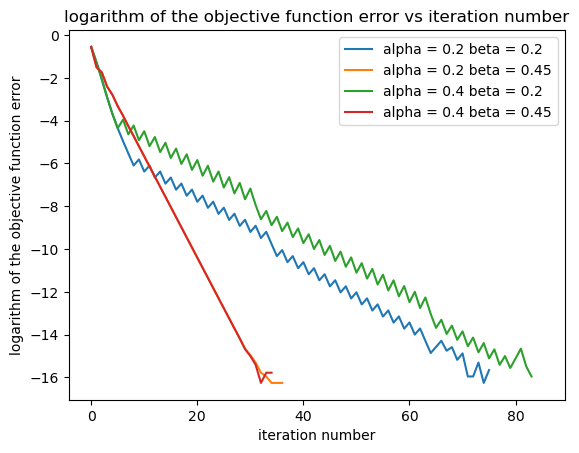
\includegraphics[width=\linewidth]{9_30_a_obj_func.png}
	\caption{Gradient descent: $f - p^*$ vs. iteration number}
\end{figure}

\begin{figure}[H]
	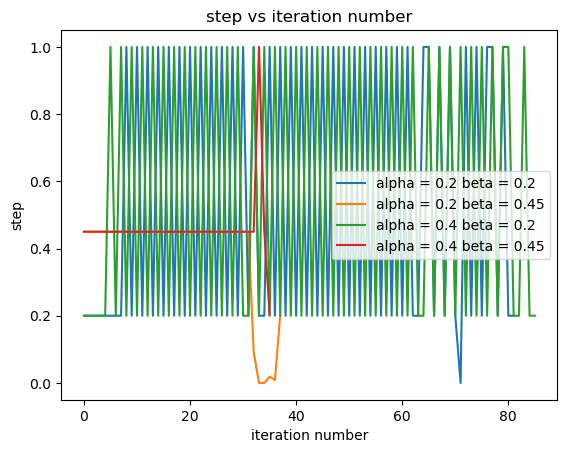
\includegraphics[width=\linewidth]{9_30_a_step.png}
	\caption{Gradient descent: step size vs. iteration number}
\end{figure}

(a) Newton's method. The python code: \\

file  \verb|ex_9_30_test_hessian.py|

\begin{verbatim}	
# -*- coding: utf-8 -*-
# https://docs.scipy.org/doc/scipy/reference/generated/scipy.optimize.check_grad.html

import numpy as np

def backtrack(x, a, grad, alpha, beta):
"""
Backtracking line search
https://stackoverflow.com/questions/52204231/implementing-backtracking-line-search-algorithm-for-unconstrained-optimization-p
"""    
t = 1
while True: 
fx = f(x - t * grad, a)
fxx = f(x, a) + alpha * t * np.dot(grad.T, grad)
if np.isnan(fx) or np.isnan(fxx):
#  print('backtrack: nan detected; multilying t: t = ', t)
t *= beta
elif fx > fxx:
t *= beta
#  print('backtrack: multilying t: t = ', t)
else: 
#  print('backtrack: t found, returning: t = ', t)
return t


def backtrack_2(x, a, grad, ihess, alpha, beta):
"""
Backtracking line search
https://stackoverflow.com/questions/52204231/implementing-backtracking-line-search-algorithm-for-unconstrained-optimization-p
"""
"""    
print('grad.shape = ', grad.shape)
print('grad = ', grad)
print('ihess.shape = ', ihess.shape)
print('ihess = ', ihess)
"""
gh = grad.T @ ihess
#  print('grad.T @ ihess = ', gh)


t = 1
while True: 
#  print('x = ', x)
#  print('gh = ', gh)

fx = f(x - t * gh , a)

fxx = f(x, a) + alpha * t * np.sum(gh ** 2)
#  fxx = f(x, a) + alpha * t * np.dot(gh, gh.T) #  the same as f(x, a) + alpha * t * np.sum(gh ** 2)

if np.isnan(fx) or np.isnan(fxx):
#  print('backtrack: nan detected; multilying t: t = ', t)
t *= beta
elif fx > fxx:
t *= beta
#  print('backtrack: multilying t: t = ', t)
else: 
#  print('backtrack: t found, returning: t = ', t)
return t

def L2norm(x):
return np.sqrt(np.sum(x ** 2))


def derivative_numerical(f, x0, i, delta = 1e-8):
xi_plus = x0.copy()
xi_plus[i] += delta

xi_minus = x0.copy()
xi_minus[i] -= delta
return (f(xi_plus) - f(xi_minus)) / (2 * delta)



def gradient_numerical(f, x0, delta = 1e-8):
"""
function calculates the numerical gradient for function f in 
the point x0
"""
N = len(x0)
grad_num = np.zeros([N, 1])
for i in range(N):
grad_num[i] = derivative_numerical(f, x0, i, delta)
return grad_num


def check_grad(f, gradf, x0, delta = 1e-8, verbose = True):
grad = np.array(gradf(x0))
grad_num = gradient_numerical(f, x0, delta)
if (verbose):
print('check_grad: precise gradient = ', grad)
print('check_grad: approximate gradient = ', grad_num)
print('check_grad: gradient error = ', grad - grad_num)        

return np.sqrt(np.sum((grad - grad_num) ** 2))

def second_derivative_numerical(f, x0, i, k, delta = 1e-5):
"""
function calculates second derivative
returns d^2f/(dx_k dx_i)
"""
xk_plus = x0.copy()
xk_plus[k] += delta

xk_minus = x0.copy()
xk_minus[k] -= delta

dfi_plus = derivative_numerical(f, xk_plus, i, delta)
dfi_minus = derivative_numerical(f, xk_minus, i, delta)

return (dfi_plus - dfi_minus) / (2 * delta)

def hessian_numerical(f, x0, delta = 1e-5):
"""
#  function calculates the hessian matrix
"""
assert x.shape[1] == 1, 'hessian_numerical: input array should have shape [N, 1]'

N = len(x)
hessian = np.zeros([N, N], dtype = np.float64)
for i in range(N):
for k in range(i, N):
hessian[i, k] = second_derivative_numerical(f, x0, i, k, delta)
if i != k:
hessian[k, i] = hessian[i, k]
return hessian

def check_hessian(f, hess_analytical, x0, delta = 1e-5, verbose = True):
"""
function checks he hessian matrix
"""
hessian_analytical = np.array(hess_analytical)
hessian_num = hessian_numerical(f, x0, delta)
if verbose:
print('check_hessian: hessian_analytical = ', hessian_analytical)
print('check_hessian: hessian_num = ', hessian_num)
print('check_hessian: hessian difference = ', 
hessian_analytical - hessian_num)

return np.sqrt(np.sum((hessian_analytical - hessian_num) ** 2))

#%%
# definitions for the function, gradient and hessian

def f(x, a):
#  calculation of the function value
if not np.all(a.T @ x < 1):
return np.nan
if not np.all(np.abs(x) <= 1):
return np.nan
ret1 = 0.0
ret1 = - np.sum(np.log(1 - a.T @ x))  
ret2 =  - np.sum(np.log(1 - np.square(x)))
return ret1 + ret2

#  print('f(x, a) = ', f(x, a))

def gradf(x, a):
#  calculation of the function gradient

if not np.all(a.T @ x < 1):
return np.nan
if not np.all(np.abs(x) <= 1):
return np.nan
#  print('x = ', x)

ret1 = 0.0    
ret1 = a @ (1 / (1 - a.T @ x))
ret2 = 2 * x * (1 / (1 - x ** 2))
return ret1 + ret2

def hessf(x, a):
if not np.all(a.T @ x < 1):
return np.nan
if not np.all(np.abs(x) <= 1):
return np.nan
ret1 = 0
ret1 = a @ (a.T * (1 / (1 - a.T @ x) ** 2))
ret2 = 2 * (1 + x ** 2) / ((1 - x ** 2) ** 2)
ret2 = np.diagflat(ret2)

return ret1 + ret2


if __name__ == "__main__":

np.random.seed(1)

m, n = 3, 2

a = np.random.random([m, n]).T

#  a = np.array([[-1, 0], [0.5, - 0.5], [0.5, 0]], dtype = np.float64).T

x0 = 0.5 * np.ones([n, 1]) 
x = np.array([-0.25, 0.75], dtype = np.float64).reshape(- 1, 1)



print('a.shape = ', a.shape)


#  x = np.array([0.5, 0.75])

#x = np.array([-0.75, 0.5], dtype = np.float64).reshape(- 1, 1)

error1 = check_grad(lambda x: f(x, a), lambda x: gradf(x, a), x0)

assert error1 < 1e-6, 'error1 too big'

print('gradient error1 = ', error1)


x0 = - 0.5 * np.ones([n, 1]) 
fl3 = lambda x: (x[0]**2 + 3*x[1]*x[0] + 12)

def f3(x):
return (x[0]**2 + 3*x[1]*x[0] + 12)[0]

dfx1 = lambda x: (2*x[0] + 3*x[1])
dfx2 = lambda x: (3*x[0])

def gradf3(x):
return np.array([dfx1(x), dfx2(x)]).reshape([-1, 1])


error3 = check_grad(f3, gradf3, x0)

print('gradient error3 = ', error3)

assert error3 < 1e-6, 'error3 too big'

error4 = check_grad(f3, gradf3, x0)

print('gradient error4 = ', error4)

assert error4 < 1e-6, 'error4 too big'

#%%
# test function for hessian 

def fh(z):
assert z.shape[0] == 2 and z.shape[1] == 1, 'fh(x): incorrect input shape'

x = z[0]
y = z[1]

return x**2 + 0.5 * y**2 + 2 * x * y + 3 * x + 4 * x**2 * y**2 + 5 * y * x**2

def fh_hessian(z):
assert z.shape[0] == 2 and z.shape[1] == 1, 'fh_hessian(x): incorrect input shape'

x = z[0]
y = z[1]

hessian = np.zeros([2, 2], dtype = np.float64)
print('')
hessian[0, 0] = 2 + 8 * y**2 + 10 * y
hessian[0, 1] = 2 + 16 * x * y + 10 * x
hessian[1, 0] = hessian[0, 1]
hessian[1, 1] = 1 + 8 * x ** 2
return hessian

#%%


#  test check_hessian function:

x0 = np.array([0.5, 8], dtype=np.float64).reshape(-1, 1)

#  x0 = np.array([0, 0], dtype=np.float64).reshape(-1, 1)

#  x0 = np.array([1, 1], dtype=np.float64).reshape(-1, 1)

hess_analytical = fh_hessian(x0)


hd = check_hessian(fh, hess_analytical, x0, delta = 1e-5, verbose = True)

print('test of check_hessian, diff = %e' % hd)

# x0 = np.array([0.5, -0.25], dtype=np.float64).reshape(-1, 1)    
x0 = np.array([-0.5, -0.75], dtype=np.float64).reshape(-1, 1)    

v_hess_analytical = hessf(x0, a)

print('v_hess_analytical = ', v_hess_analytical)


v_hess_num = hessian_numerical(lambda x: f(x, a), x0)

print('v_hess_num = ', v_hess_num)

hc = check_hessian(lambda x: f(x, a), v_hess_analytical, x0)
print('hc = ', hc)

assert hc < 1e-4, 'hessian seems to be incorrect'

grad = np.array([[3.26697727], [4.08950456]])    
ihess = np.array([[ 0.31264018, -0.13959122],  [-0.13959122,  0.28763308]])
print('grad.shape = ', grad.shape)
print('ihess.shape = ', ihess.shape)
y = grad.T @ ihess
print('y = ', y)
print('y.shape = ', y.shape)


print(np.sum(y**2))
\end{verbatim}	

file  \verb|ex_9_30_b.py|

\begin{verbatim}
# -*- coding: utf-8 -*-

import numpy as np
import ex_9_30_test_hessian as h
import matplotlib.pyplot as plt
plt.close('all')


f = h.f

np.random.seed(3)

m, n = 800, 60

a = np.random.random([m, n]).T


#  parameters for gradient descent method

nu_min = 1e-8 #  tolerance

step = 0.3

x_start = np.zeros([n, 1])

x = x_start


iter_num = 0

max_iters = 1000

max_line_search_iters = 1000

alpha = 0.4

beta = 0.4

print('x_start = ', x_start)
print('x_start.shape = ', x_start.shape)


# t = h.backtrack(x, a, h.gradf(x, a), alpha, beta)
# print('t after backtrack = ', t)

# the Newton's method implementation
while True:

print('iteration number ', iter_num)
grad = h.gradf(x, a) #  gradient of f
hess = h.hessf(x, a) #  hessian of f
ihess = np.linalg. inv(hess) #  inverse hessian of f
dx = - ihess @ grad #  Newton step
lam_sq = grad.T @ (ihess @ grad) # Newton decrement

print('lam_sq = %e' % lam_sq)
if np.sqrt(lam_sq / 2) <= nu_min:
print("Newton's method: tolerance achieved, exiting...")
print('iteration number ', iter_num)
#  print('a = ', a)
print('optimal value = %e' % f(x, a))
print('optimal x = ', x)
break
#  Backtracking line search

t = h.backtrack_2(x, a, grad, ihess, alpha, beta)
step = t
# step = 1

print('step =', step)

x = x + step * dx

print('new x = ', x)    
iter_num += 1
if iter_num >= max_iters:
print("Newton's method: max_iters number exeeded")
break


def newton_method(alpha, beta):

obj_func_arr = []
step_arr = []
iter_num = 0
x = x_start

while True:

print('iteration number ', iter_num)
obj_func_arr.append(f(x, a))
grad = h.gradf(x, a) #  gradient of f
hess = h.hessf(x, a) #  hessian of f
ihess = np.linalg. inv(hess) #  inverse hessian of f
dx = - ihess @ grad #  Newton step
lam_sq = grad.T @ (ihess @ grad) # Newton decrement

print('lam_sq = %e' % lam_sq)
#  if lam_sq / 2 <= nu_min:
if np.sqrt(lam_sq / 2) <= nu_min:
print("Newton's method: tolerance achieved, exiting...")
print('iteration number ', iter_num)
#  print('a = ', a)
opt_val = f(x, a)
print('optimal value = %e' % opt_val)
print('optimal x = ', x)
return np.array(obj_func_arr) - opt_val, step_arr            
break
#  Backtracking line search

t = h.backtrack_2(x, a, grad, ihess, alpha, beta)
step = t
step_arr.append(step)

print('step =', step)

x = x + step * dx

print('new x = ', x)    
iter_num += 1
if iter_num >= max_iters:
print("Newton's method: max_iters number exeeded")
return None, None
break

# plot the graphs        
alpha_arr = [0.2, 0.4]

beta_arr = [0.2, 0.45]

plt.figure()

for alpha in  alpha_arr:
for beta in beta_arr:
print('alpha = ', alpha)
print('beta = ', beta)
obj_func, step =  newton_method(alpha, beta)
x_plt = range(len(obj_func))
plt.plot(x_plt, np.log10(obj_func), 
label='alpha = ' + str(alpha) + ' beta = ' + str(beta))

plt.title('logarithm of the objective function error vs iteration number')
plt.ylabel('logarithm of the objective function error')
plt.xlabel('iteration number')
plt.legend()
plt.show()

plt.savefig('9_30_b_obj_func.png', bbox_inches='tight')


plt.figure()

for alpha in  alpha_arr:
for beta in beta_arr:
print('alpha = ', alpha)
print('beta = ', beta)
obj_func, step =  newton_method(alpha, beta)
x_plt = range(len(step))
plt.plot(x_plt, step, 
label='alpha = ' + str(alpha) + ' beta = ' + str(beta))

plt.title('step vs iteration number')
plt.ylabel('step')
plt.xlabel('iteration number')
plt.legend()
plt.show()

plt.savefig('9_30_b_step.png', bbox_inches='tight')
		
\end{verbatim}	

\begin{figure}[H]
	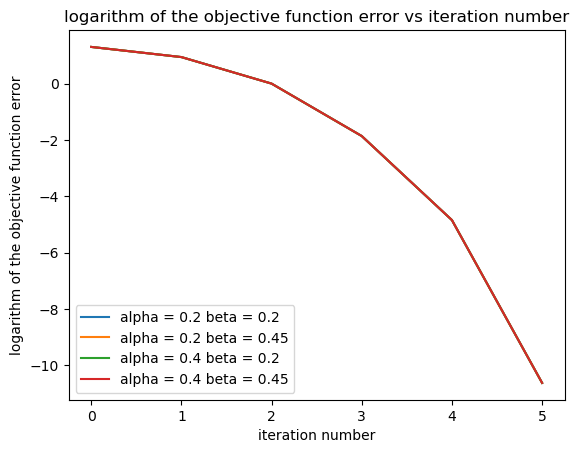
\includegraphics[width=\linewidth]{9_30_b_obj_func.png}
	\caption{Newton's method: $f - p^*$ vs. iteration number}
\end{figure}

\begin{figure}[H]
	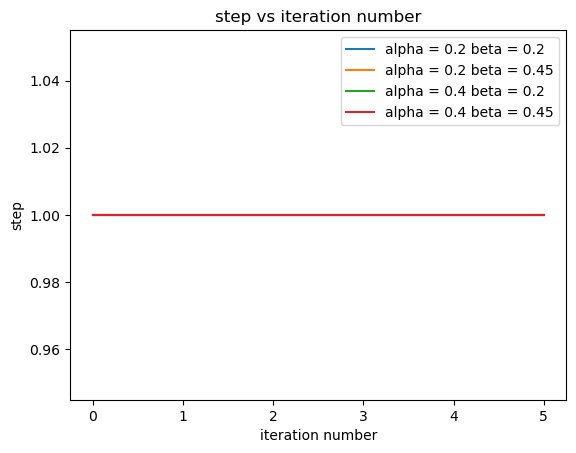
\includegraphics[width=\linewidth]{9_30_b_step.png}
	\caption{Newton's method: step size vs. iteration number}
\end{figure}


\section*{9.31}

\end{document}

